\documentclass[a4paper,12pt]{article}

\usepackage{amsfonts, amsmath, amssymb, amsthm, enumitem, fancyhdr, graphicx}
\usepackage[margin=1in, includehead, includefoot, heightrounded]{geometry}
\allowdisplaybreaks
\pagestyle{fancy}
\rhead{Erick Lin}

\DeclareMathOperator*{\argmax}{\arg\!\max}
\DeclareMathOperator*{\argmin}{\arg\!\min}
\newcommand{\norm}[1]{\left\lVert#1\right\rVert}
\renewcommand{\thesubsection}{\arabic{subsection}}
\newtheorem{theorem}{Theorem}
\newtheorem{lemma}[theorem]{Lemma}
\sloppy

\begin{document}

\section*{MATH 4640 -- HW5 Solutions}
\begin{enumerate}
    \item
        The corresponding function is $f(x) = 2 - (1 + c)x + cx^3$ which has derivative $f'(x) = -(1 + c) + 3cx^2$. For any $\varepsilon > 0$, a fixed point theorem states that if $|f'(x)| < 1$ for all $x \in [\alpha - \varepsilon, \alpha + \varepsilon]$, then $f(x)$ has exactly one fixed point (which must be $\alpha$) in the interval, and the iteration in question also converges. Letting $\varepsilon \to 0$, the condition is satisfied whenever $|f'(\alpha)| = |2c - 1| < 1$, or $0 \leq c < 1$. \par
        The convergence is quadratic if and only if $f'(\alpha) = 0$, which is true for $c = 1/2$ (otherwise, the convergence is linear). \par
        We can prove the previous fact as follows: since $|x_n - \alpha| = |f(x_{n - 1}) - f(\alpha)|$, from the Taylor series of $f(x_{n - 1})$,
        \begin{align*}
            |x_n - \alpha| &= \left| \frac{f'(\alpha)}{1!}(x_{n - 1} - \alpha) + \frac{f''(\alpha)}{2!} (x_{n - 1} - \alpha)^2 + \frac{f'''(\alpha)}{3!}(x_{n - 1} - \alpha)^3 + \cdots \right| \\
            &= O(x_{n - 1} - \alpha)^2
        \end{align*}
        if and only if $f'(\alpha) = 0$.

    \item
        \begin{enumerate}
            \item
                The corresponding function is $f(x) = -16 + 6x + \frac{12}{x}$, which has derivative $f'(x) = 6 - \frac{12}{x^2}$. We have that $|f'(\alpha)| = |6 - \frac{12}{2^2}| = 3 \geq 1$, so from the fixed point theorem, the iteration does not converge on any interval containing $\alpha$.
            \item
                The corresponding function is $f(x) = \frac{2}{3}x + \frac{1}{x^2}$, which has derivative $f'(x) = \frac{2}{3} - \frac{2}{x^3}$. We have that $|f'(\alpha)| = |{\frac{2}{3}} - \frac{2}{3}| = 0 < 1$, so from the fixed point theorem, the iteration converges if $x_0$ is close enough to $\alpha$. The convergence is quadratic because $|f'(\alpha)| = 0$.
            \item
                The corresponding function is $f(x) = \frac{12}{1 + x}$, which has derivative $f'(x) = -\frac{12}{(1 + x)^2}$. We have that $|f'(\alpha)| = |{-\frac{12}{(1 + 3)^2}}| < 1$, so from the fixed point theorem, the iteration converges if $x_0$ is close enough to $\alpha$. The convergence is linear because $|f'(\alpha)| \neq 0$.
        \end{enumerate}

    \item
        $n = 3$:
        \begin{gather*}
            A_3 =
            \left[ \begin{array}{ccc}
                2 &-1 &0 \\
                -1 &2 &-1 \\
                0 &-1 &2
            \end{array} \right]
            \xrightarrow{R_2 \rightarrow R_2 + \frac{1}{2}R_1}
            \left[ \begin{array}{ccc}
                2 &-1 &0 \\
                0 &\frac{3}{2} &-1 \\
                0 &-1 &2
            \end{array} \right]
            \xrightarrow{R_3 \rightarrow R_3 + \frac{2}{3}R_2}
            \left[ \begin{array}{ccc}
                2 &-1 &0 \\
                0 &\frac{3}{2} &-1 \\
                0 &0 &\frac{4}{3}
            \end{array} \right]
            = U \\
            L = \left[ \begin{array}{ccc}
                    1 & 0 & 0 \\
                    -\frac{1}{2} & 1 & 0 \\
                    0 & -\frac{2}{3} & 1
            \end{array} \right]
        \end{gather*}
        $n = 4$:
        \begin{gather*}
            A_4 =
            \left[ \begin{array}{cccc}
                2 &-1 &0 &0 \\
                -1 &2 &-1 &0 \\
                0 &-1 &2 &-1 \\
                0 &0 &-1 &2
            \end{array} \right]
            \xrightarrow{R_2 \rightarrow R_2 + \frac{1}{2}R_1}
            \left[ \begin{array}{cccc}
                2 &-1 &0 &0 \\
                0 &\frac{3}{2} &-1 &0 \\
                0 &-1 &2 &-1 \\
                0 &0 &-1 &2
            \end{array} \right] \\
            \xrightarrow{R_3 \rightarrow R_3 + \frac{2}{3}R_2}
            \left[ \begin{array}{cccc}
                2 &-1 &0 &0 \\
                0 &\frac{3}{2} &-1 &0 \\
                0 &0 &\frac{4}{3} &-1 \\
                0 &0 &-1 &2
            \end{array} \right]
            \xrightarrow{R_4 \rightarrow R_4 + \frac{3}{4}R_3}
            \left[ \begin{array}{cccc}
                2 &-1 &0 &0 \\
                0 &\frac{3}{2} &-1 &0 \\
                0 &0 &\frac{4}{3} &-1 \\
                0 &0 &0 &\frac{5}{4}
            \end{array} \right] = U \\
            L = \left[ \begin{array}{cccc}
                    1 & 0 & 0 & 0 \\
                    -\frac{1}{2} & 1 & 0 & 0 \\
                    0 & -\frac{2}{3} & 1 & 0 \\
                    0 & 0 & -\frac{3}{4} & 1
            \end{array} \right]
        \end{gather*}
        Guess:
        \begin{gather*}
            A_n =
            \left[ \begin{array}{ccccc}
                    1 & 0 & \cdots & \cdots & 0 \\
                    -\frac{1}{2} & 1 & \cdots & \cdots & \vdots \\
                    0 & -\frac{2}{3} & 1 & \cdots & \vdots \\
                    \vdots & \ddots & \ddots & \ddots & 0 \\
                    0 & 0 & 0 & -\frac{n}{n + 1} & 1 \\
            \end{array} \right]
            \left[ \begin{array}{cccccc}
                    2 & -1 & 0 & \cdots & \cdots & 0 \\
                    0 & \frac{3}{2} & -1 & 0 & \cdots & \vdots \\
                    \vdots & 0 & \frac{4}{3} & \ddots & \ddots & \vdots \\
                    \vdots & \vdots & 0 & \ddots & \ddots & 0 \\
                    \vdots & \vdots & \vdots & \ddots & \ddots & -1 \\
                    0 & 0 & \cdots & \cdots & 0 & \frac{n + 1}{n}
            \end{array} \right] = LU
        \end{gather*}
        Verification: \\
        $A_{i, i} = \sum_{k = 1}^n L_{i, k} U_{k, i} = (-\frac{i - 1}{i})(-1) + \frac{i + 1}{i} = \frac{i - 1}{i} + \frac{i + 1}{i} = \frac{2i}{i} = 2$ for all $1 \leq i \leq n$, \\
        $A_{i - 1, i} = \sum_{k = 1}^n L_{i - 1, k} U_{k, i} = 1(-1) = -1$ for all $2 \leq i \leq n$, \\
        $A_{i, i - 1} = \sum_{k = 1}^n L_{i, k} U_{k, i - 1} = -\frac{i - 1}{i} \frac{i}{i - 1} = -1$ for all $2 \leq i \leq n$, \\
        $A_{i, j} = 0$ for all $|i - j| > 1$. \par
        Thus, $A_n = LU$ is the correct factorization.

    \item
        With \texttt{A} and \texttt{b} initialized as expected, the plot of the norm of the error resulting from running
        \begin{center}
            \texttt{x = jacobi(A, b, 0.001)} \\
            \texttt{jacobi(A, b, 0.001, x)} \\
        \end{center}
        is below:
        \begin{center}
            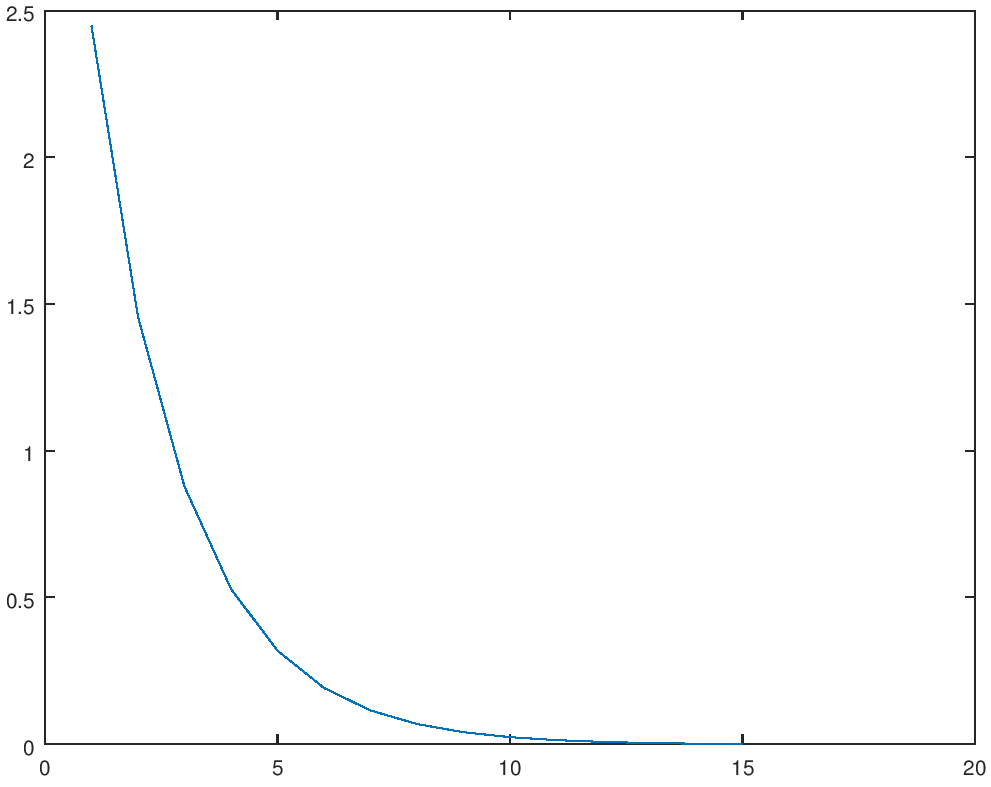
\includegraphics[scale=0.25]{jacobi_error}
        \end{center}

    \item
        The plot of the norm of the error resulting from running
        \begin{center}
            \texttt{x = gauss\_seidel(A, b, 0.001)} \\
            \texttt{gauss\_seidel(A, b, 0.001, x)} \\
        \end{center}
        is below:
        \begin{center}
            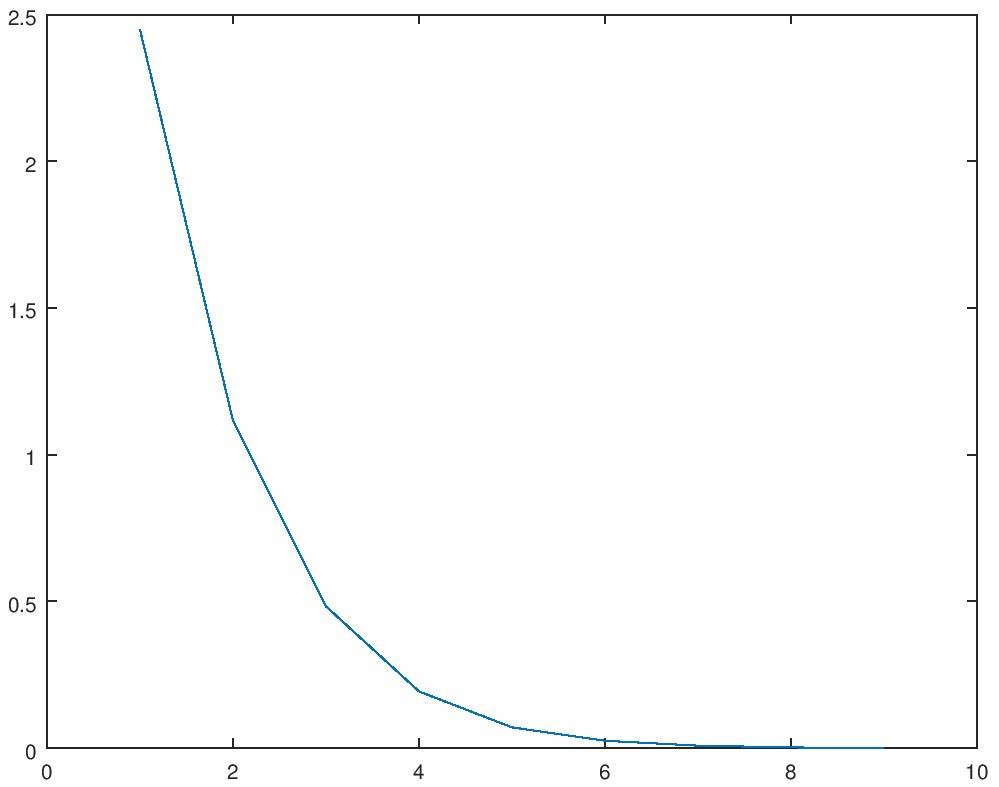
\includegraphics[scale=0.25]{gauss_seidel_error}
        \end{center}

    \item
        Initializing \texttt{A} as expected and letting \texttt{v\_0} be the zero vector, running
        \begin{center}
            \texttt{[v, lambda] = power\_method(A, v\_0, 1)}
        \end{center}
        allows us to determine that the eigenvalue-eigenvector pair is
        \begin{align*}
            (\lambda, \vec{v}) = (15, [0.5, 0.5, 0.5, 0.5]^T),
        \end{align*}
        as we have that $A\vec{v} = \lambda\vec{v} = [7.5, 7.5, 7.5, 7.5]^T$.
\end{enumerate}

\end{document}
